\subsection{Infinite Horizon LQR Formulierung}
    Der LQ-Regler beruht auf einem intuitiven Ansatz bei dem man beliebig einen Trade-off zwischen Regelfehler und Regelaufwand wählt. 
    
    LQR ist eine Abkürzung für \textit{linear quadratic regulator}. 
    
    \textbf{Linear:} da das System linear ist:
    \[\frac{d}{dt}x(t) = A\cdot x(t) + B\cdot u(t),\ x(t) \in \mathbb{R}^n,\ u(t) \in \mathbb{R}^m\]
    \textbf{Quadratic:} Definition einer  \textit{quadratischen} Kostenfunktion J:
    \[
    \colorboxed{red}{
    J(u(t)) = \int_0^\infty\Big(x(u(t))^T\cdot Q\cdot x(u(t)) + u(t)^T \cdot R \cdot u(t)\Big)dt
    }
    \]
    der optimale Eingnang $u^*(t)$ minimiert die Kostenfunktion J:
     \[u^*(t) = \arg\min J(u(t))\]
     Die Zustände $x(t)$ und Eingänge $u(t)$ werden in Optimierungsproblem mit $Q$ und $R$ gewichtet, wobei 
     \[Q=Q^T \in \mathbb{R}^{n\times n},\ Q \succeq 0,\ \textnormal{und}\ R = R^T \in \mathbb{R}^{m\times m},\ R\succ 0\]
     Die Definitheit der Matrizen $Q$ und $R$ ist notwendig, damit das Argument des Integrals quadratisch konvex ist.
     Somit ist das Minimum von $J(u)$ einzigartig, falls es existiert.
    
    \textbf{Regulator:}
    der Reglerlösst das \textit{regulator} Problem:
    \[\lim\limits_{t \to \infty}x(t)=0\]
    
    $\boxed{Q\uparrow \widehat{=}\, R \downarrow}$ \textbf{Cheap Control.} Je grösser $Q$ relativ zu $R$, desto teurer ist es wenn $x(t)$ nicht im Ursprung ist. Das System wird schnell an den Ursprung geregelt, um die Kosten tiefstmöglich zu halten. Dabei wird $u(t)$ jedoch betragsmässig gross sein.
    
    $\boxed{Q\downarrow \widehat{=}\, R \uparrow}$ Je grösser $R$ relativ zu $Q$, desto teurer ist es viel Energie mit den Ausgangsgrössen auszugeben. Das System wird langsam (mit betragsmässig kleinem Regelsignal $u(t)$) in den Ursprung geregelt.
    
    \textbf{Note:} eine Erhöhung der Eigenwerte von $Q$ hat den gleichen Effekt wie eine Reduzierung derer von $R$. Die relative Grösse ist von Relevanz.
    
    \subsubsection{Lösung der LQR-Formulierung}
        Die Lösung der LQR-Formulierung ist eine \textbf{lineare Zustandsrückführung} und lautet  
        \[
        \colorboxed{red}{
        u^*(t) = -K\cdot x(t),\ \textnormal{wobei}\ K = R^{-1}\cdot B^T\cdot\Phi
        }
        \]
        
        Note: Die Matrix $K$ ist \textbf{statisch}, sie muss für gegebene $\{A,B,Q,R\}$ nur einmal berechnet werden.
    
    \subsubsection{algebraische Riccati Gleichung}
        Dabei ist $\Phi$ die einzige positive Lösung der algebraischen Riccati Gleichung 
        \begin{equation*}
        \colorboxed{red}{
        \Phi\cdot B \cdot R^{-1}\cdot B^T \cdot \Phi-\Phi \cdot A - A^T \cdot \Phi - Q = 0
        }
        \end{equation*}
        
        Wählt man 
        \[Q = \overline{C}^T\cdot \overline{C},\quad \overline{C}\in\mathbb{R}^{p\times n}\ \textnormal{wobei}\ p = \operatorname{rank}(Q),\]
        dann ist $\Phi$ garantiert positiv definit, falls $\{A,B\}$ \textbf{steuerbar} und $\{A,\Bar{C}\}$ \textbf{beobachtbar} sind. Diese Bedingungen sind hinreichen aber nicht notwendig.
        
        Note:
        \begin{enumerate}
            \item  Die Matrix $\overline{C}$ hat nichts mit der Matrix C zu tun. Falls jedoch $\overline{C} = C$ gewählt wird, wird $||y(t)||_2$ in der Kostenfunktion berücksichtigt.
            \item Der open loop gain lautet $L_{LQR}(s) = K\cdot (sI-A)^{-1}\cdot B$ 
            \begin{figure}[H]
                \centering
                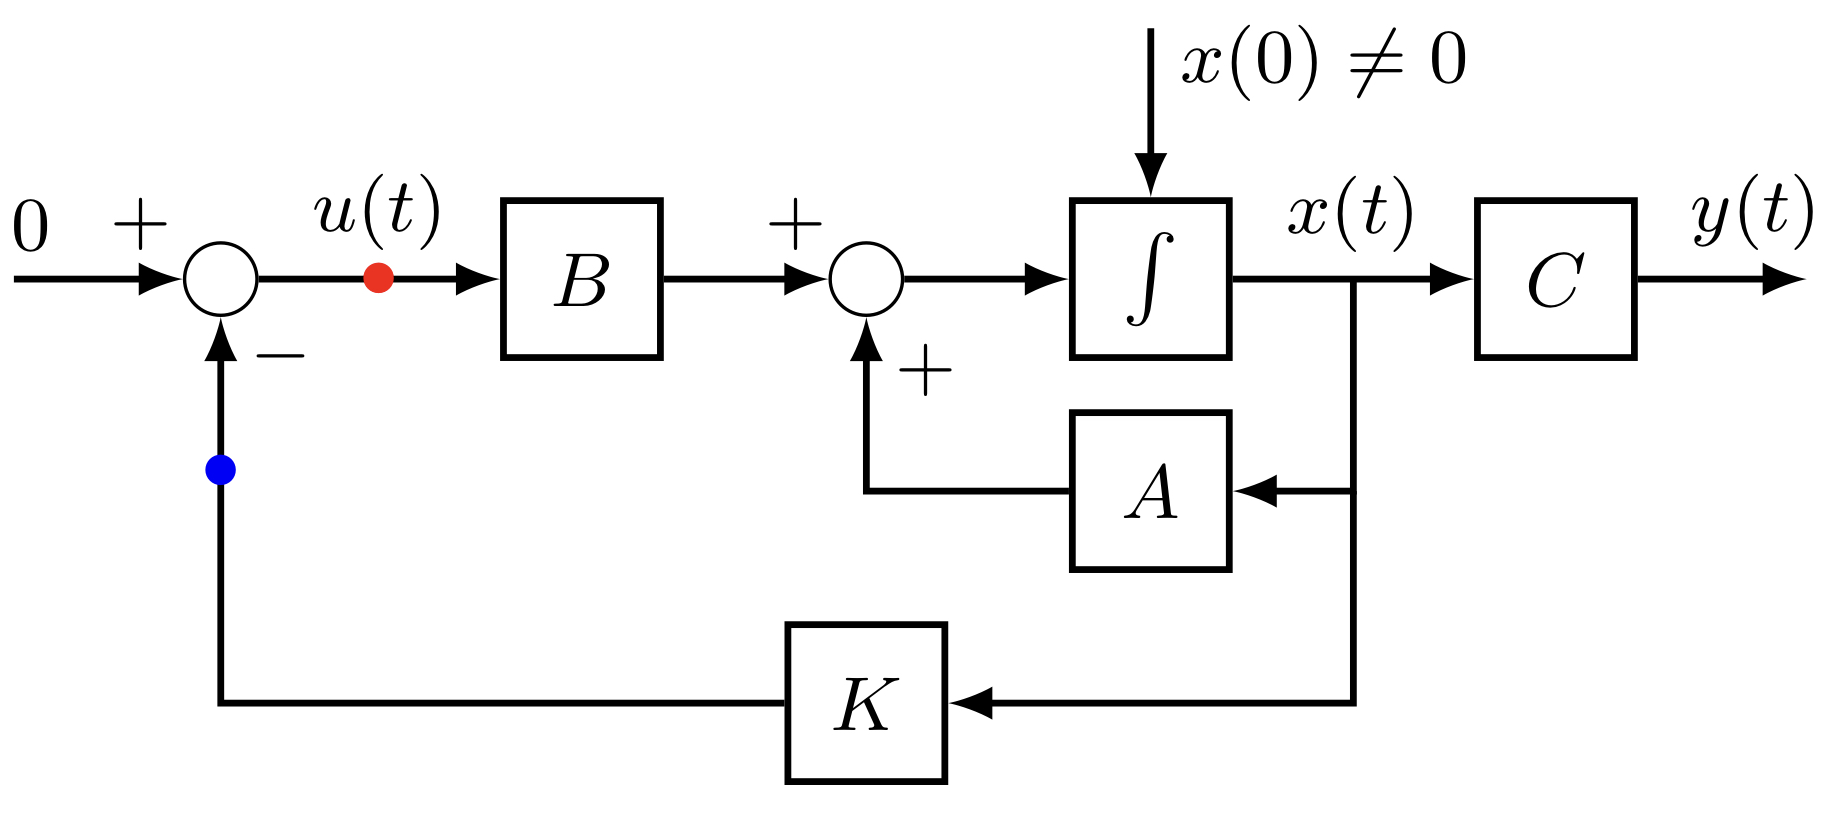
\includegraphics[width = 0.5\linewidth]{08/L_lqr.jpeg}
                \caption{$L_{\textnormal{LQR}}$ von $\textcolor{red}{\bullet}  \rightarrow \textcolor{blue}{\bullet}$}
            \end{figure}
            \item Robust Stability ist auch bei Modellunsicherheit gewährleistet.
        \end{enumerate}
    
    \subsubsection{Eigenschaften von Infinite Horizon Reglern}
        \textbf{Stabilität:}
        Die Matrix $A-B\cdot K$ des geschlossenen Regelkreises ist \textbf{garantiert Hurwitz} (stabil).
        \begin{equation*}
            \colorboxed{red}{\Dot{x}(t) = \big(A - B\cdot K\big) \cdot x(t)}
        \end{equation*}
    
        \textbf{Robustheit:}
        Für die Wahl $R=r\cdot I$ hat die minimum return difference $\mu_{min}$ folgende Eigenschaft:\[\mu_{min,LQR} = \min_{\omega}\Big(\min_{i}\ \sigma_i(I+L_{LQR}(j\omega))\Big) \geq 1 \]
        
        Im SISO-Fall lässt sich diese Eigenschaft folgendermassen darstellen.
        Dies garantiert eine Verstärkungsreserve von $\gamma \in [\,0.5, \infty)$ und eine Phasenreserve von $\varphi \geq 60^\circ$
        
        \begin{figure}[H]
            \centering
            \includegraphics[width=0.5\linewidth]{08/SISO_Robustheit.jpg}
            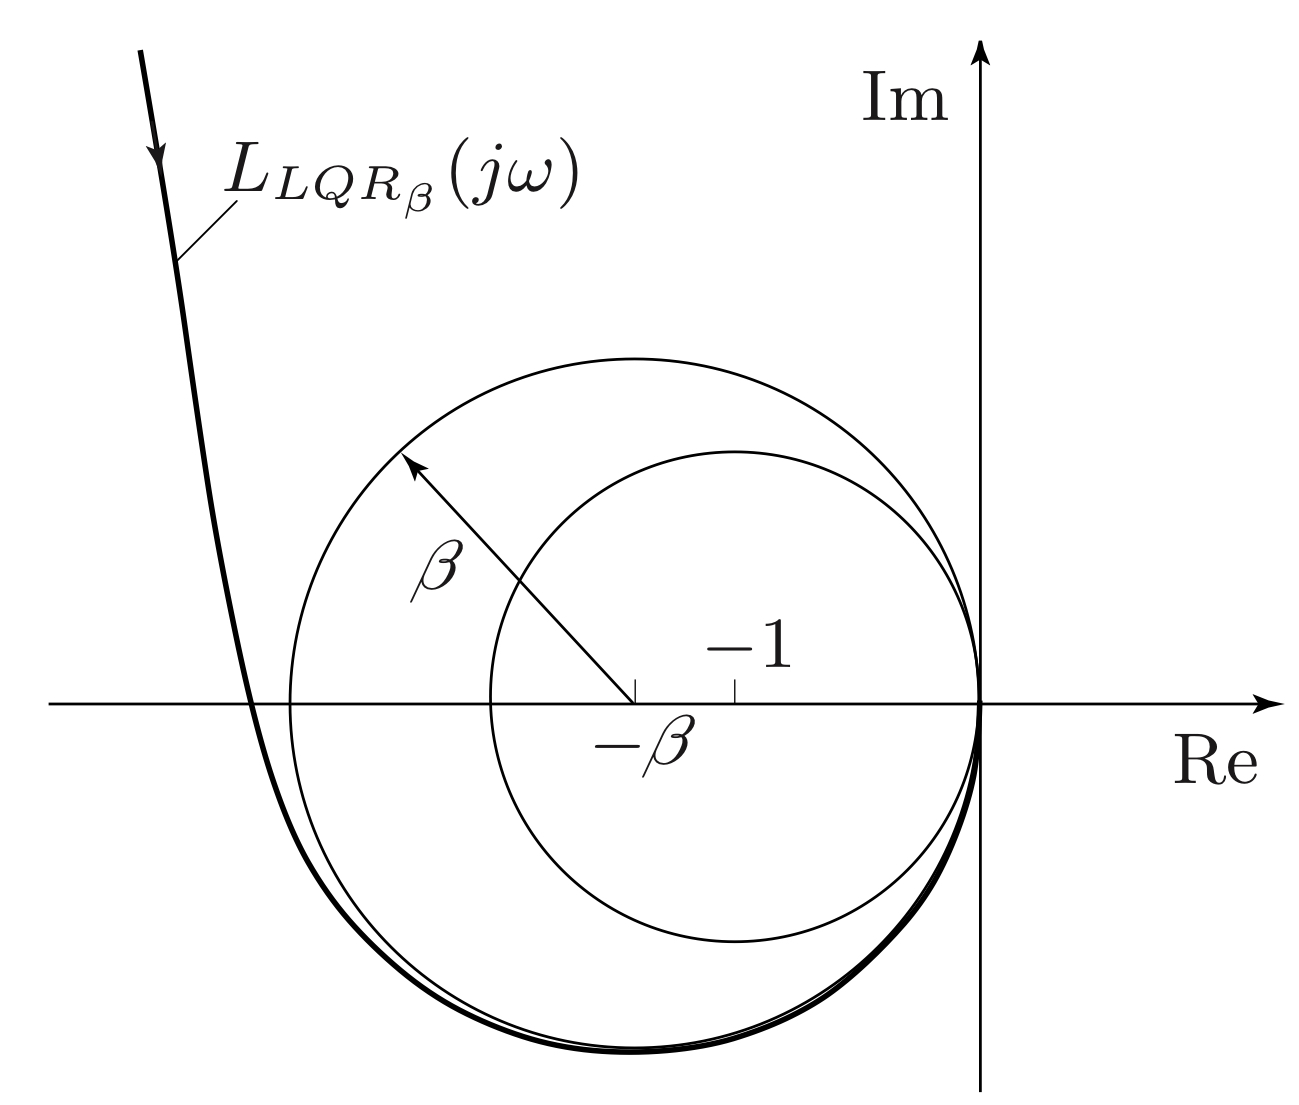
\includegraphics[width=0.4\linewidth]{08/beta_robust.jpeg} 
        \end{figure}
        % \begin{figure}[H]
        %     \centering
        %     \includegraphics[width = 0.6 \linewidth]{images/08/SISO_Robustheit.jpg}
        % \end{figure}
    
        Durch modifizieren der Riccati-Gleichung mit $\beta > 1$ wie folgt:
        \[\frac{1}{\beta}\cdot\Phi_\beta\cdot B\cdot R^{-1}\cdot B^T\cdot \Phi_\beta - \Phi_\beta \cdot A - A^T\cdot \Phi_\beta-Q = 0\]
        
        so resultiert die Lösung $\Phi_\beta$. Damit wird der Regelkreis noch robuster, da dann gilt: 
        
        \[\mu_{min,LQR}=\min_\omega\Big(\min_{i}\ \sigma_i(\beta I+L_{LQR}(j\omega))\Big) \geq \beta \]
        
        Das heisst, der Nyquist-Plot tritt nie in den um $-\beta +j\cdot0$ zentrierten Kreis mit Radius $\beta$ ein.
        